\subsection{Results} The online experiment was performed outside of our
control, and some participants quit the experiment prematurely.  In
total we had 105 subjects (13 offline, 92 online) starting the survey,
of those 93 completed the preliminary questionnaire, and 84, 71, 65,
and 56 subjects started respectively T1, T2, T3 and T4.  All of the
subjects in the offline setting started all tasks.
Figure~\ref{fig:resultPerTask} shows the outcome of the tasks; in the 
remainder of this section consider only the outcomes marked as ``Correct''.

\begin{figure}[t]
    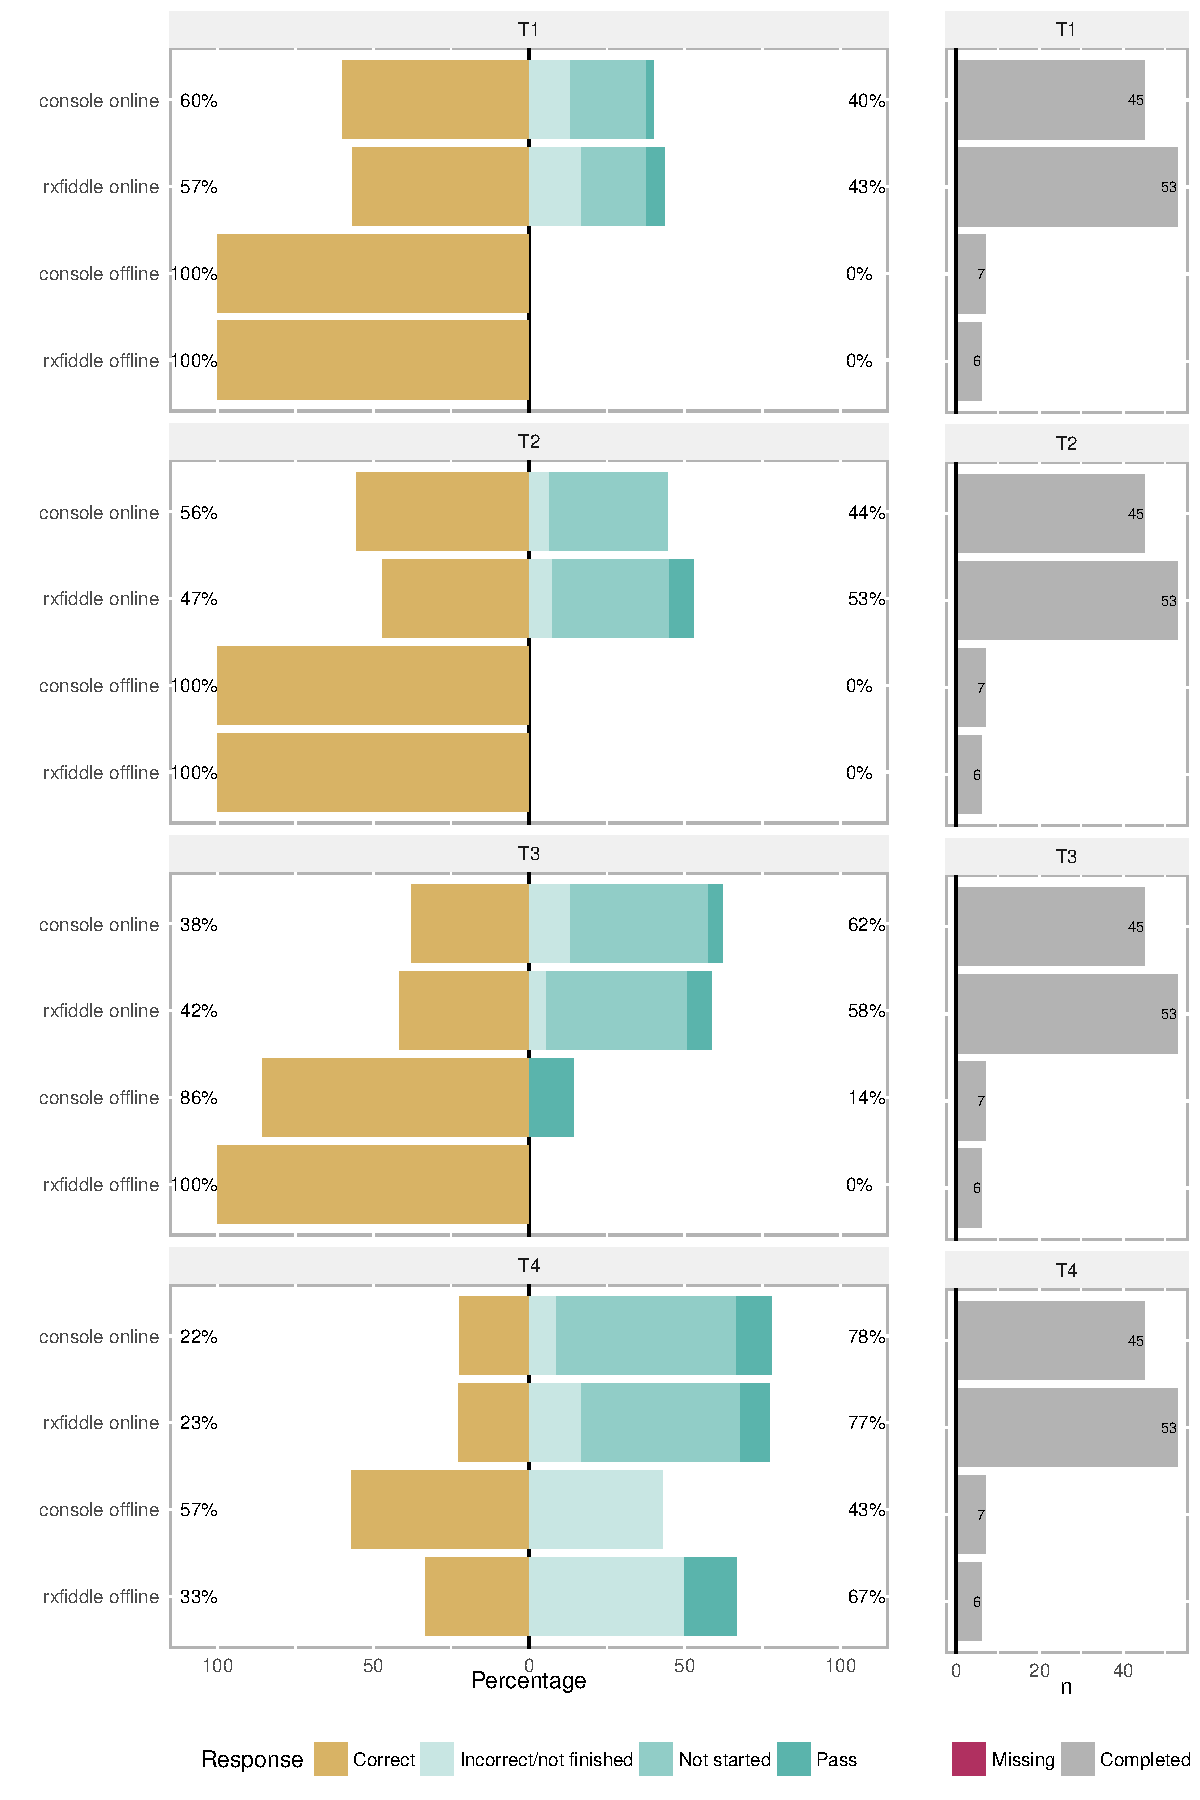
\includegraphics[width=\columnwidth]{images/resultPerTask.pdf}
    \caption{Task outcome per group (RxFiddle/Console) and environment (online/offline)}
    \label{fig:resultPerTask}
\end{figure}

\paragraph{Overall} Figure~\ref{fig:timePerTask} 
shows the time until the correct answer was given
per task.  Here we consider the combined results from the offline experiment
and the online experiment.  We make no assumptions about the underlying
distribution so we perform a non-parametric Wilcoxon Mann-Whitney U test
(\textit{$ H_0 $:  times for the Console group and RxFiddle group are
drawn from the same population}) to see if the differences are
significant, and a Cliff's delta test for ordinal data to determine the
effect size. The results are shown in Table~\ref{table:result}.

\begin{table}[h!]
    {\centering% \begin{table}[]
% \centering
% \caption{My caption}
%\label{my-label}
\begin{tabular}{llllll}
\hline
            & \textbf{$n_1$} & \textbf{$n_2$} & \textbf{W} & \textbf{p-value} & \textbf{Cliffs $\delta$} \\ \hline
\textbf{T1} & 26                      & 30                       & 343        & 0.448           & 0.121     \\
\textbf{T2} & 29                      & 27                       & 362        & 0.637           & 0.0754    \\
\textbf{T3} & 22                      & 24                       & 100        & 0.000186        & 0.621     \\
\textbf{T4} & 15                      & 12                       & 86         & 0.867           & 0.0444    \\ \hline
\end{tabular}
% \end{table}}
    \caption{Results comparing the Console and RxFiddle groups, with 
    respectively $n_1$ and $n_2$ subjects.}
    \label{table:result}
\end{table}

For tasks T3 we can reject $ H_0 $ with high significance ($ p < 0.05 $),
\emph{the RxFiddle group is faster}.  For the tasks T1, T2 and T4 we can
not reject $ H_0 $ ($ p > 0.05 $), meaning the \emph{RxFiddle group and
Console group perform or could perform equally}.

\begin{figure}[t]
    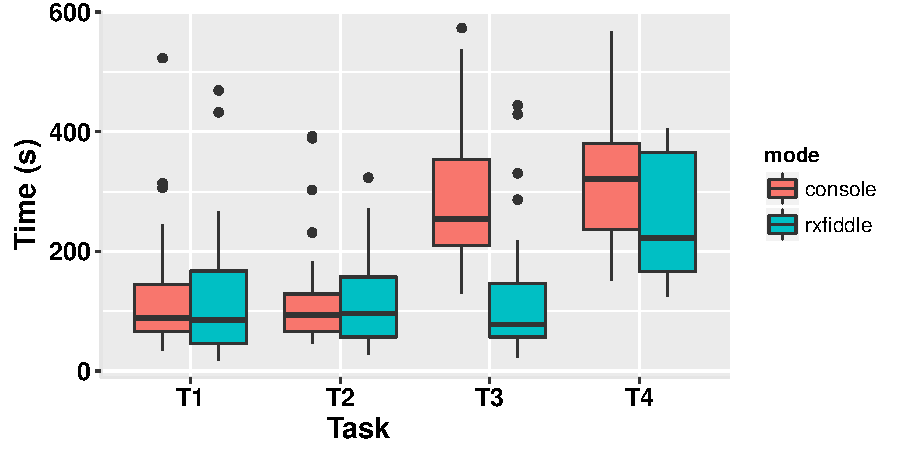
\includegraphics[width=\columnwidth]{images/timePerTask.pdf}
    \caption{Time until correct answer per task, overall}%
    \label{fig:timePerTask}
\end{figure}

\paragraph{Control for experience} To investigate this further, we split
the results for different groups of subjects, as shown in Figure~%
\ref{fig:timePerTaskSplit} in the Appendix.  When we control for the
self-assessed Rx experience, we see bigger differences for all tasks for groups
with more experience, as shown in Figure~%
\ref{fig:timePerTaskRx} and Table~\ref{table:result-split} (we split at the 
median value; greater than ``Beginner''-level).

\begin{table}[t]
    {\centering\begin{tabular}{llllll}
    \hline
                & \textbf{$n_1$} & \textbf{$n_2$} & \textbf{W} & \textbf{p-value} & \textbf{Cliff's $\delta$} \\
    \hline
    \textbf{T1} & 16             & 17             & 105        & 0.276            & 0.228                     \\
    \textbf{T2} & 14             & 13             & 99         & 0.720            & -0.0879                   \\
    \textbf{T3} & 10             & 11             & 10         & $7.88e^{-4}$     & 0.818                     \\
    \textbf{T4} & 8              & 7              & 13         & $9.34e^{-2}$     & 0.536                     \\
    \hline
\end{tabular}}
    \caption{Results comparing the Console and RxFiddle groups, with 
    respectively $n_1$ and $n_2$ subjects, with Rx experience above 
    ``Beginner''-level.}
    \label{table:result-split}
\end{table}

\begin{figure}[t]
    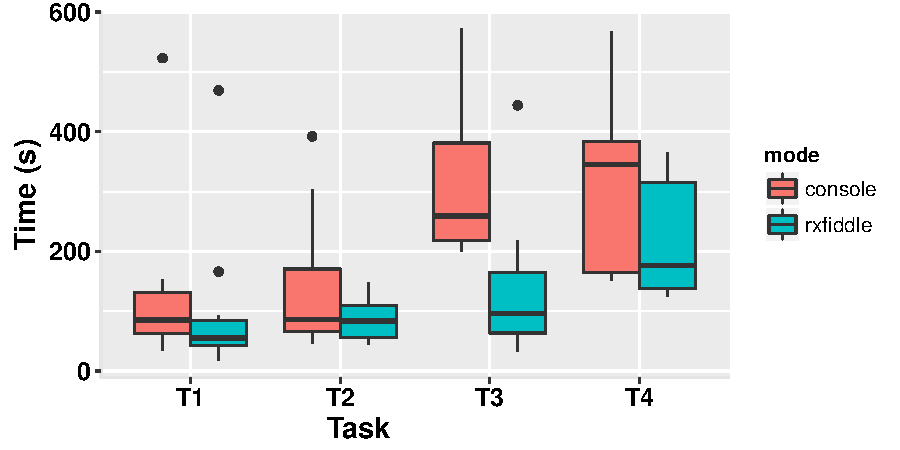
\includegraphics[width=\columnwidth]{images/timePerTaskRx.pdf}
    \caption{Time until correct answer per task, for subjects with more
    than ``Beginner''-level of experience with Rx}%
    \label{fig:timePerTaskRx}
\end{figure}

Still, for tasks T1, T2, and T4 we can not reject $ H_0 $, but the
results are more significant comparing only experienced subjects.
